\chapter{Background}
\label{chap:backgroud}

In this chapter, we will introduce some basic terminology as well as provide further information surrounding carbon scheduling.

\section{The Composition of the Public Grid}

As outlined in the previous chapter, the energy production of the public grid is supplied by different producers.
Renewables create order of magnitudes less emissions than conventional technologies.  

\begin{table}[h!]
    \centering
    \begin{tabular}{|c|c|}
    \hline
        Technology & gCO\textsubscript{2}/kWh \\ \hline
        Nuclear & 5 \\ \hline
        Hydro, Wind & 12 \\ \hline
        Solar & 35 \\ \hline
        Gas & 530 \\ \hline
        Coal & 1079 \\ \hline
    \end{tabular}
    \caption{The carbon intensity of different energy sources.\webcite{web_electricitymaps}}
    \label{tab:carbon_intensities}
\end{table}

As supply and demand in power need to be balanced, the composition of the grid changes according to changes in demand.
On the day scale, there are at least two dimensions to this. For once, there is the aforementioned diurnal rhythm of solar production.\todo{I also wanted to mention the duck curve, or how there are changes to demand from human patterns.}

In addition to that, there is also a seasonal effect on the energy grid composition:
As shown in Figure \ref{fig:energy_mix_year}, during warm seasons (e.g. July), more solar is produced than in colder seasons and the share in renewables rises accordingly.

\begin{figure}
    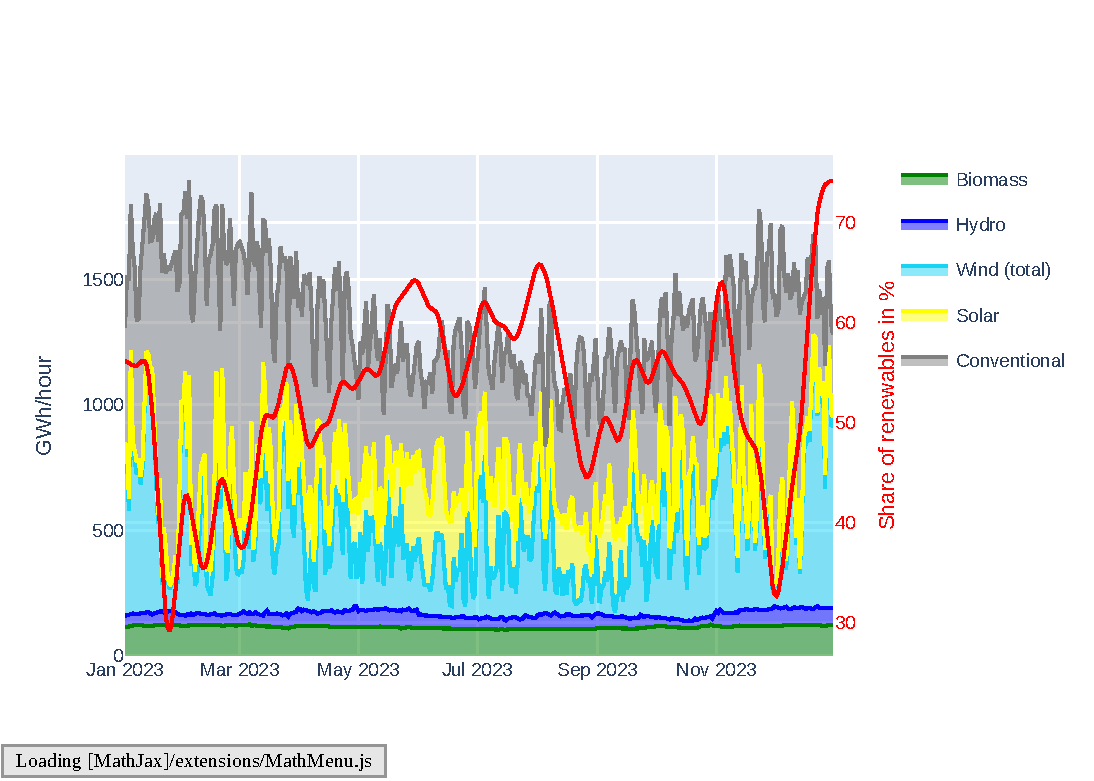
\includegraphics[width=\linewidth]{agorameter/energy_production_year.pdf}
    \caption[short]{Mix of energy production in Germany in 2023 \webcite{web_agora}. Seasonally, renewables will be highest during summer but may also spike during holidays. Thus, yearly time scopes can also be considered for carbon-aware scheduling.}
    \label{fig:energy_mix_year}
\end{figure}

The power demand also affects the overall composition. 
During times of low demand, less conventional power needs to be produced and renewables have a higher share as well.
This can be seen in the seasonal Figure: during the Christmas holidays in December, people spend more time at home, requiring less overall energy and less conventional power needs to be produced.

All of the above is a local or national view on the public grid. 
When looking at energy production globally, a spatial dimension is added. 
This takes effect in the form of different countries having peak solar production at different times (following the earth's rotation) but also takes effect in the composition of production capabilities.
Some countries may have less investment in renewables or use nuclear power plants, which are also deemed low-carbon\todo{Needs citation} but have less of a seasonal or daily rhythm (if they are not limited by lack of cooling water \webcite{noauthor_heatwave_2023}).

Thus, national public grids have a certain affinity for carbon-aware scheduling\cite{wiesner_lets_2021}. Generally, the higher the solar capacities, the higher the potential carbon saving from such an approach. 

\section{Power Grid Signals}
Carbon-aware scheduling commonly uses one of two possible metrics or signals: \emph{average emissions} are the metric describing the amount of carbon per unit of energy. These are calculated using the weighted average of all power supplies at a point.

Another metric is \emph{marginal emissions}. 
This uses a causal approach between deciding to use power and the carbon emissions associated with producing that power\webcite{web_elec_marginal}.
Marginal emissions are closely related to the way energy producers in- or decrease production:
To reduce electricity prices, additional demand on the grid is dispatched to the cheapest power plant with remaining capacity.
These power plants, also called \emph{marginal power plants}, correlate with emissions. 
An example is provided in Figure \ref{fig:marginal_example}. 
With the cheapest power coming from renewables, additional demand is supplied with more expensive, more carbon-intensive, conventional power plants.

\begin{figure}
    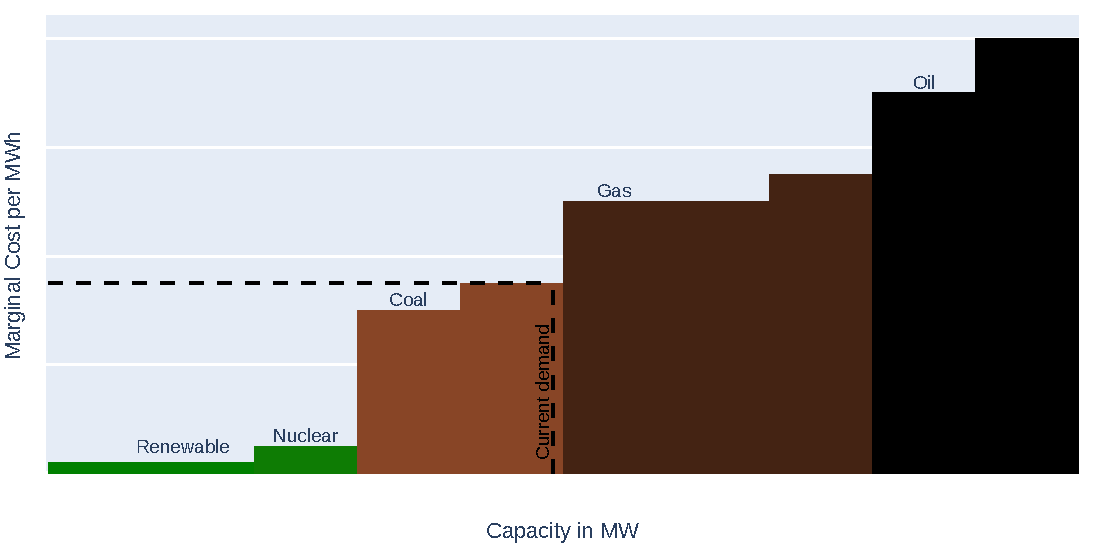
\includegraphics[width=\linewidth]{notebooks/marginal_emissions.pdf}
    \caption[short]{
        Idealized energy grid showcasing the mechanics of the marginal emissions signal. 
        Additional demand is dispatched to the cheapest plant with remaining capacity. 
        In this example, increased demand will be dispatched to a, not yet utilized, gas plant.
        Thus, the individual decision to increase demand \emph{now} is reflected in high marginal emissions.
        The costs and carbon emissions are loosely follow \webcite{web_costs_energy_production} and \webcite{web_ipcc_emissions} 
        }
    \label{fig:marginal_example}
\end{figure}

Two providers of signal data are \emph{Electricitymaps}\webcite{web_electricitymaps} and \emph{WattTime}\webcite{web_watttime}.
Electricitymaps has a free access API for historical and current average emissions. Both providers only offer the marginal signal commercially, however. 

From here on, the average signal will be used. 
Note that current literature is still split on which signal is best. 
A recently released by Sukprasert et al. \cite{sukprasert_limitations_2024} may be read for further information on grid signals and arguments for either signal.

One reason for using the average signal is \emph{curtailment}. 
Curtailment encompasses any methods that reduce production of renewable energy. As the power grid always needs to have a balance between demand and production, curtailment methods such as turning off wind turbines, selling power at a loss, or charging batteries may be used. 
Carbon-aware scheduling via the average emissions signal lowers the amount of curtailment needed, because otherwise left-over renewables get utilized due to better matching demand.
Another argument made, for example by Fridgen et al. \cite{fridgen_not_2021}, is that by increasing power demand during times when renewable production is high, investments in renewables would be promoted. 
Lastly, as renewable energy is generally cheaper in production than non-renewable energy\todo{Need a citation here!}, scheduling work on low carbon periods coincides with cheaper energy prices as well. While this would not reduce costs on most energy contracts, some contracts do use dynamic pricing.\webcite{web_tibber}

\paragraph{Workloads in a Datacenter} According to Tanenbaum and Woodhull\cite{tanenbaum_operating_2006}, there are three environments in which scheduling may take place. \emph{Batch systems} describe environments in which there is no user interaction. 
Scientific simulations and computations, machine learning workloads, and data processing tasks are examples of such workloads\cite{sukprasert_limitations_2024}. 
A user may submit their job, and it would be executed according to the scheduler at some point in time. 
On the contrary, in \emph{interactive} settings, a user interacts with the system and thus expects quick responses to their inputs. 
An example of interactive workloads are web requests. In a recent work by Souza et al. \cite{souza_casper_2024}, they can be answered carbon-awarely by using a spatially distributed cloud services, dispatching requests to regions with lower carbon intensity. 
Locally, the carbon-emissions of LLM inferences, which are used in chatbot applications, can be reduced as shown by Hoffmann and Majunkte\cite{hoffmann_improving_2024}.\todo{Bisschen random?}
Regulations, such as the European GDPR \webcite{web_gdpr} play into this, however.
The last environment is \emph{real-time} systems. There, deadlines and predictability dictate how a scheduler operates.

For this work's topic, (temporal) carbon-aware scheduling, only batch systems will be examined as they allow more freedom when scheduling workloads.

\section{Measuring Power}

There are multiple options for measuring the power of a given computer. One way of classifying these options is categorizing them under \emph{logical measurements} or \emph{physical measurements}.

Logical ones create a model on some metrics and derive the used power. One example is using Linux's \emph{perf} tool to read hardware performance counters, then assigning an energy cost to select counters and multiplying that. 

Advantages of choosing a logical approach are that no external hardware is needed and that the overhead of the measurement is low, as the hardware counters are being kept track of anyway. 
Disadvantages on the other hand are that such a model has to be created or chosen and includes some form of error as all models do.

Physical measurements follow another route; measurement devices are put between the operating hardware and the power supply. 
The point where a power measuring device is inserted dictates what could and could not be measured, a wall-mounted measurement device could only measure all power going into a computer and not differentiate between individual programs.

The advantages of physical measurements are that they can give a more holistic measurement of a system as would be the case for a wall-mounted measurement device. 
Portability is an issue: unlike operating-system supported tools such as perf, a measurement device needs more effort to be used on another system (or be entirely unusable, for example when such devices are only rated for a certain power level).

% \paragraph{Power Consumption of a Computer}
% As there will be power measurements in \ref{sec:power_measurements}, some basic understanding of energy and power used for computation will be provided:
% \begin{itemize}
%     \item I could mostly borrow from the EBRH slides; there is some base power needed that is correlated to the hardware (dynamic and static energy)
%     \item this also depends on frequency (which is why later we set our CPU frequency to some hard coded value [or do not do that in the case of my GPU lol])
%     \item basically, use this paragraph to outline all things we take care of in my power measurements
% \end{itemize}